% Standard Article Definition
\documentclass[]{article}

% Page Formatting
\usepackage[margin=1in]{geometry}
\setlength\parindent{0pt}

% Graphics
\usepackage{graphicx}

% Math Packages
\usepackage{physics}
\usepackage{amsmath, amsfonts, amssymb, amsthm}
\usepackage{mathtools}

% Extra Packages
\usepackage{pdfpages}
\usepackage{hyperref}
% \usepackage{listings}

% Section Heading Settings
% \usepackage{enumitem}
% \renewcommand{\theenumi}{\alph{enumi}}
\renewcommand*{\thesection}{Problem \arabic{section}}
\renewcommand*{\thesubsection}{\arabic{section}\alph{subsection})}
\renewcommand*{\thesubsubsection}{}%\quad \quad \roman{subsubsection})}

\newcommand{\Problem}{\subsubsection*{\textbf{PROBLEM:}}}
\newcommand{\Solution}{\subsubsection*{\textbf{SOLUTION:}}}
\newcommand{\Preliminaries}{\subsubsection*{\textbf{PRELIMINARIES:}}}

%Custom Commands
\newcommand{\N}{\mathbb{N}}
\newcommand{\Z}{\mathbb{Z}}
% \newcommand{\Q}{\mathbb{Q}}
\newcommand{\R}{\mathbb{R}}
\newcommand{\C}{\mathbb{C}}

% \newcommand{\SigAlg}{\mathcal{S}}

% \newcommand{\Rel}{\mathcal{R}}

% \newcommand{\toI}{\xrightarrow{\textsf{\tiny I}}}
% \newcommand{\toS}{\xrightarrow{\textsf{\tiny S}}}
% \newcommand{\toB}{\xrightarrow{\textsf{\tiny B}}}

% \newcommand{\divisible}{ \ \vdots \ }
\newcommand{\st}{\ : \ }

% Theorem Definition
% \newtheorem{definition}{Definition}
% \newtheorem{assumption}{Assumption}
% \newtheorem{theorem}{Theorem}
% \newtheorem{lemma}{Lemma}
% \newtheorem{proposition}{Proposition}
% \newtheorem{remark}{Remark}
% \newtheorem{example}{Example}
% \newtheorem{counterExample}{Counter Example}


%opening
\title{
    MECH 6v29 - Model Predictive Control\\ 
    Homework 3
}
\author{Jonas Wagner\\ jonas.wagner@utdallas.edu}
\date{2023, October 20\textsuperscript{th}}

\begin{document}

\maketitle

\tableofcontents

%% Problem 1
\newpage
\section{}
Problem Data:

% 1a)
\subsection{}
Problem Data:
\begin{equation}
    \begin{aligned}
        \mathbf{A} = \mqty[1&1\\0&1] & \mathbf{B} = \mqty[0.5\\1] & \mathcal{W} = \{\vb{w} = \mathbf{B} z \st \abs{z} \leq 0.3\}\\
        \mathbf{C} = \mqty[1&0\\1&0\\0&0] & \mathbf{D} = \mqty[0\\0\\1] & \mathcal{Y} = \{\vb{y} \in \R^3 \st \norm{\vb{y}}_{\infty} \leq 1\}
    \end{aligned}
\end{equation}

Prediction Horizon:
$N = 10$

Initial Condition:
$\vb{x}_0 = \mqty[0\\0]$

% 1b)
\subsection{Nilpotent candidate controller}
$\Lambda(\mathbf{A+BK}) = 0$

Result w/ Acker:
$\vb{K} = \mqty[-1 & -1.5]$

Same as in \cite{}.


% 1c)
\subsection{Output constraint tightening}
From reference (using different notation):
\begin{equation}
    \begin{aligned}
        \mathcal{Y}_0 = \mathcal{Y}\\
        \mathcal{Y}_{j+1} = \mathcal{Y}_{j} \ominus (\mathbf{C + DK}) \mathbf{L}_{j} \mathcal{W}, \quad \forall_{j \in \{0,\dots,N-1\}}
    \end{aligned}
\end{equation}
where $\mathbf{L}_{j} = (\mathbf{A+BK})^{j}$.\footnote{not explicitly, but eliminating time-variance that's what it is...}

Or equivalently, using the time-invarience of K and some version of the Cayley-Hamilton theorem, 
\begin{equation}
    \mathcal{Y}_{j} = \mathcal{Y} \ominus \bigoplus_{i = 1,\dots,n} (\mathbf{C+DK}) (\mathbf{A+BK})^{i-1}
\end{equation}
(eliminating if the power is negative...)

TODO: double check this... (pretty sure this falls under some distributed property...)

For this system,
$(\mathbf{C+DK}) = \mqty[\vb{I}_2\\\mathbf{K}]$

\begin{equation}
    \begin{aligned}
        \mathcal{Y}_0 &= \{\vb{y} \in \R^3 \st \norm{\vb{y}}_{\infty}\leq 1\}\\
            &= \{\vb{y} \in \R^{3} \st \abs{y_1} \leq 1, \abs{y_2} \leq 1, \abs{y_3}\leq 1\}\\
        \mathcal{Y}_1 &= \mathcal{Y}_0 \ominus (\mathbf{C+DK}) \mathcal{W}\\
            &= \mathcal{Y}_0 \ominus \mqty[\vb{I}_2\\\mathbf{K}] \{ \vb{B} w \in \R \st \abs{w} \leq 0.3\}\\
            &= \{\vb{y} \in \R^{3} \st \abs{y_1} \leq 0.85, \abs{y_2} \leq 0.7, \abs{y_3}\leq 0.4\}\\
        \mathcal{Y}_1 &= \mathcal{Y}_1 \ominus (\mathbf{C+DK}) \mathbf{(A+BK)}\mathcal{W}\\
            &= \mathcal{Y}_1 \ominus \mqty[\vb{I}_2\\\mathbf{K}] \{\vb{B} w \in \R \st \abs{w} \leq 0.3\}\\
            &= \{\vb{y} \in \R^{3} \st \abs{y_1} \leq 0.7, \abs{y_2} \leq 0.4, \abs{y_3}\leq 0.1\}\\
    \end{aligned}
\end{equation}
which is the same for the remaining since $(\mathbf{A+BK})^2 = \vb{0}$.

































%% Problem 2
\newpage
\section{}
Problem Data:
\begin{equation}
    \begin{aligned}
        \mathbf{A} = \mqty[1&1\\0&1] & \mathbf{B} = \mqty[0.5\\1] & \mathcal{W} = \{\vb{w} = \mathbf{B} z \st \abs{z} \leq 0.3\}\\
        \mathbf{C} = \mqty[1&0\\1&0\\0&0] & \mathbf{D} = \mqty[0\\0\\1] & \mathcal{Y} = \{\vb{y} \in \R^3 \st \norm{\vb{y}}_{\infty} \leq 1\}
    \end{aligned}
\end{equation}

Prediction Horizon:
$N = 10$

Initial Condition:
$\vb{x}_0 = \mqty[0\\0]$

Candidate Feedback Controller:
$K = \mqty[-1 & -1.5]$

% 1a)
\subsection{Set Definitions}
\textbf{State/Input Constraints:}
From the output constraints the individual state/input constraints can be found by satisfying
$C \mathcal{X} = \mathcal{Y} \ominus D \mathcal{U}$
and 
$D \mathcal{U} = \mathcal{Y} \ominus C \mathcal{X}$;
but $C$ and $D$ would have to be invertible for a direct solution, so I'm not sure if it's good.

TODO: double check this...

Alternatively, we can look at the individual dimensions/values and do it simply by observation as we can decompose the dimensions:
\begin{equation}
    \begin{aligned}
        \mathcal{X} &= \{x \in \R^n \st \norm{C x}_\infty \leq 1\} 
            = \{x \in \R^n \st \abs{x_1} \leq 1, \ \abs{x_2} \leq 1\}\\
        \mathcal{U} &= \{u \in \R^m \st \norm{D u}_\infty \leq 1\}
            = \{u \in \R^m \st \abs{u_1} \leq 1\}
    \end{aligned}
\end{equation}

In H-rep this becomes:
\begin{equation}
    \begin{aligned}
        \mathcal{X} &= \qty{A = \mqty[\vb{I}_2\\-\vb{I}_2], \ b = \mqty[1\\1]}\\
        \mathcal{U} &= \qty{A = \mqty[1\\-1], \ b = \mqty[1\\1]}
    \end{aligned}
\end{equation}

\textbf{Disturbance Set:}
$\mathcal{W}$ is defined by 
\begin{equation}
    \mathcal{W} = \{\vb{w} = \mathbf{B} z \st \abs{z} \leq 0.3\}
\end{equation}
and in H-rep it becomes
\begin{equation}
    \mathcal{W} = \qty{A = \mqty[B\\-B], \ b = \mqty[0.3\\0.3]}
\end{equation}

\newpage
% 2b)
\subsection{RPI Sets}
Constructing the RPI set was done in MATLAB following process in provided code (as instructed):
\begin{figure}[h]
    \centering
    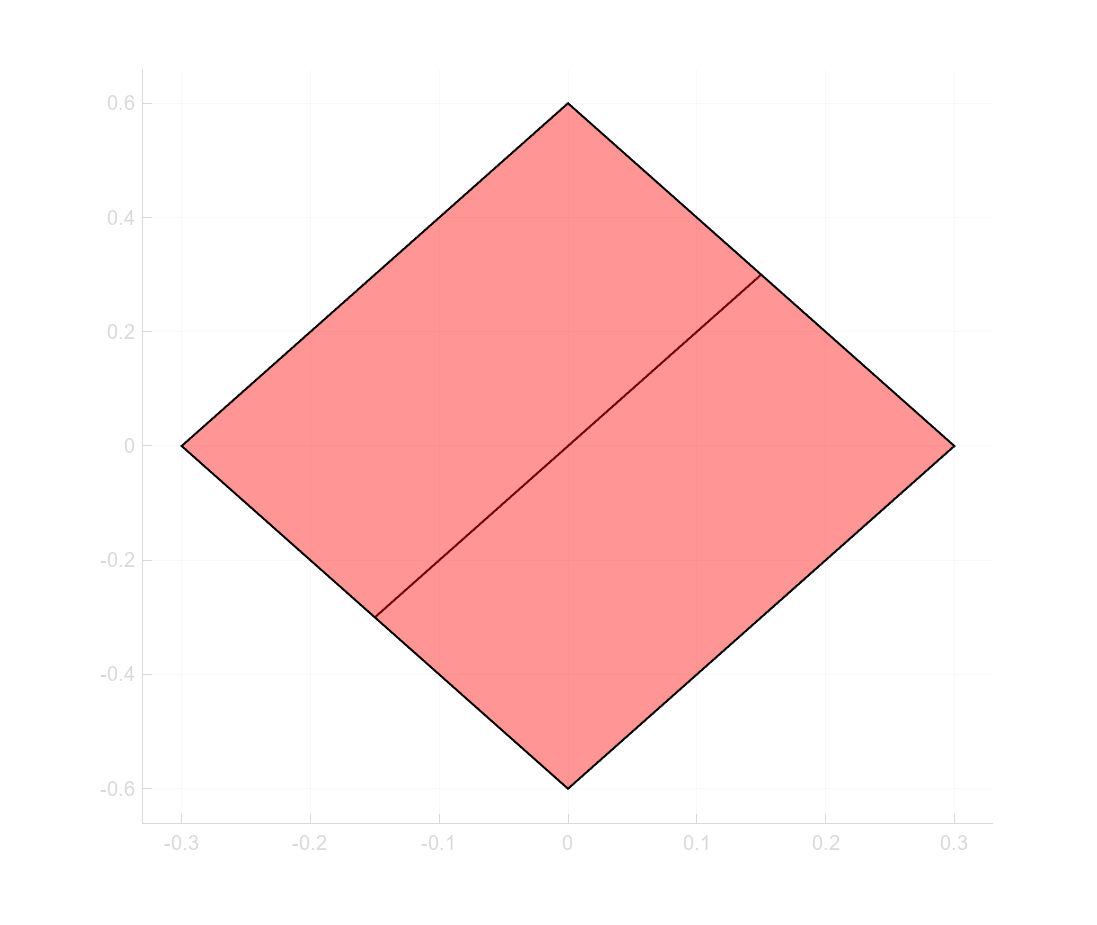
\includegraphics[width=0.5\textwidth]{figs/pblm2b_1.png}\\
    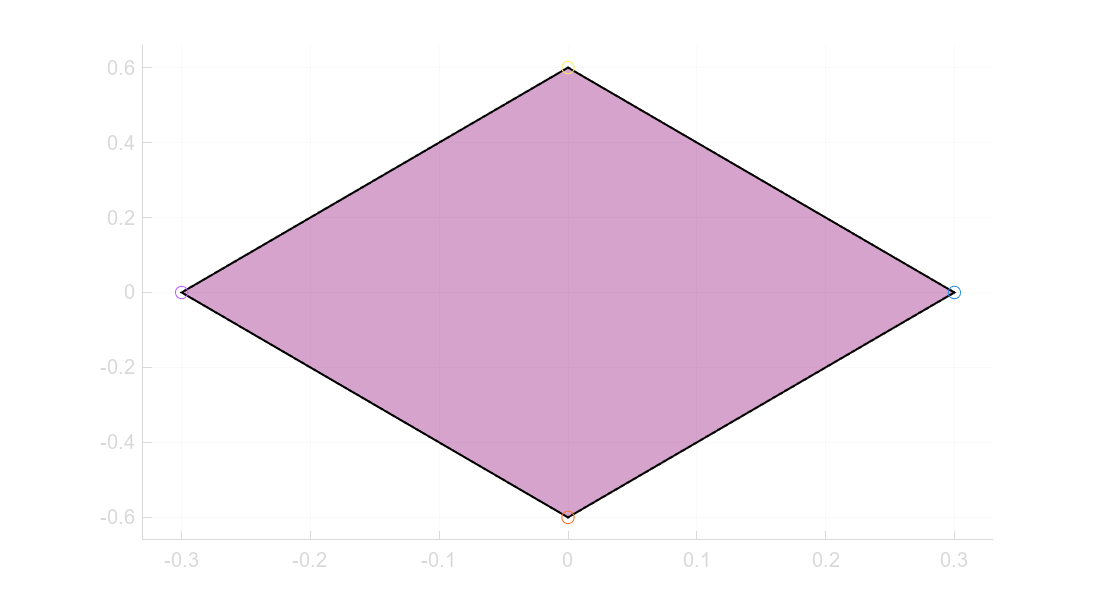
\includegraphics[width=0.5\textwidth]{figs/pblm2b_2.png}
    \caption{First one is the iterative portion and the second one is the one using the provided Approx\_RPI() function}
\end{figure}

Testing different epsilon values resulted in an RPI set that didn't look all that different and the vertices all appeared to line up. 
(Tested many epsilon values all less than 1)

The result of $Z$ is calculated in MATLAB as:
\begin{equation}
    Z = \mqty[
        0.8639  & -0.4319 & 0.2592 \\
        0.8639  & 0.4319  & 0.2592 \\
        -0.8639 & 0.4319  & 0.2592 \\
        -0.8639 & -0.4319 & 0.2592 ]
\end{equation}

\newpage
% 2c)
\subsection{Tightened Input/Output Constraint Sets}
From \cite{}, the disturbance invarient set for $x_{k+1} = A_K x_k + w$ is defined by $A_K Z \oplus W \subseteq Z$, where $A_K = A + B*K$ is stable.

This $Z$ is the RPI set for $x_{k+1} = A_K x_k + w$.
The proposition from the reference says that if $x_k \in \bar{x}_k$ and $u_k \in \bar{u}_k + K(x - \bar{x})$, then $x_{k+1} \in \bar{x}_{k+1} \oplus Z$ $\forall_{w_k \in W}$.
Where $x_{k+1} = A x_{k} + B u_{k} + w_k$. 
\footnote{some of the time-invarience isn't included}

Result makes it so that $u_k = \bar{u}_k + K (x_k = \bar{x}_k)$ keeps the state close to the nominal one.
\footnote{this also means it can ensure that it satisfies state/input constraints as well}

The new state and input constraints are based on $Z_k$ for each time-step.

To ensure that $x^*_k = x_k \oplus Z$ satisfies the original constraint set, the new constraints of 
\begin{equation}
    \bar{\mathcal{X}} = \mathcal{X} \ominus Z = \qty{x \in \R^2 \st \abs{x_1} \leq 0.7, \abs{x_2} \leq 0.4}
\end{equation}

For the input, the state constraints are satisfied as 
\begin{equation}
    \bar{\mathcal{U}} = \mathcal{U} \ominus K Z = \qty{u \in \R \st \abs{u} \leq 0.1}
\end{equation}

As expected, both constraint sets are smaller than the original sets.

% 2d)
\subsection{Controller Formulation}
The controller is now described differently then before in a different way.






\newpage
\appendix
\section{Code}
\subsection{Github}
See my github repo for all my course related materials: 
\url{https://github.com/jonaswagner2826/MECH6v29_MPC}

\subsection{Matlab results}
MATLAB code and results are attached.
% 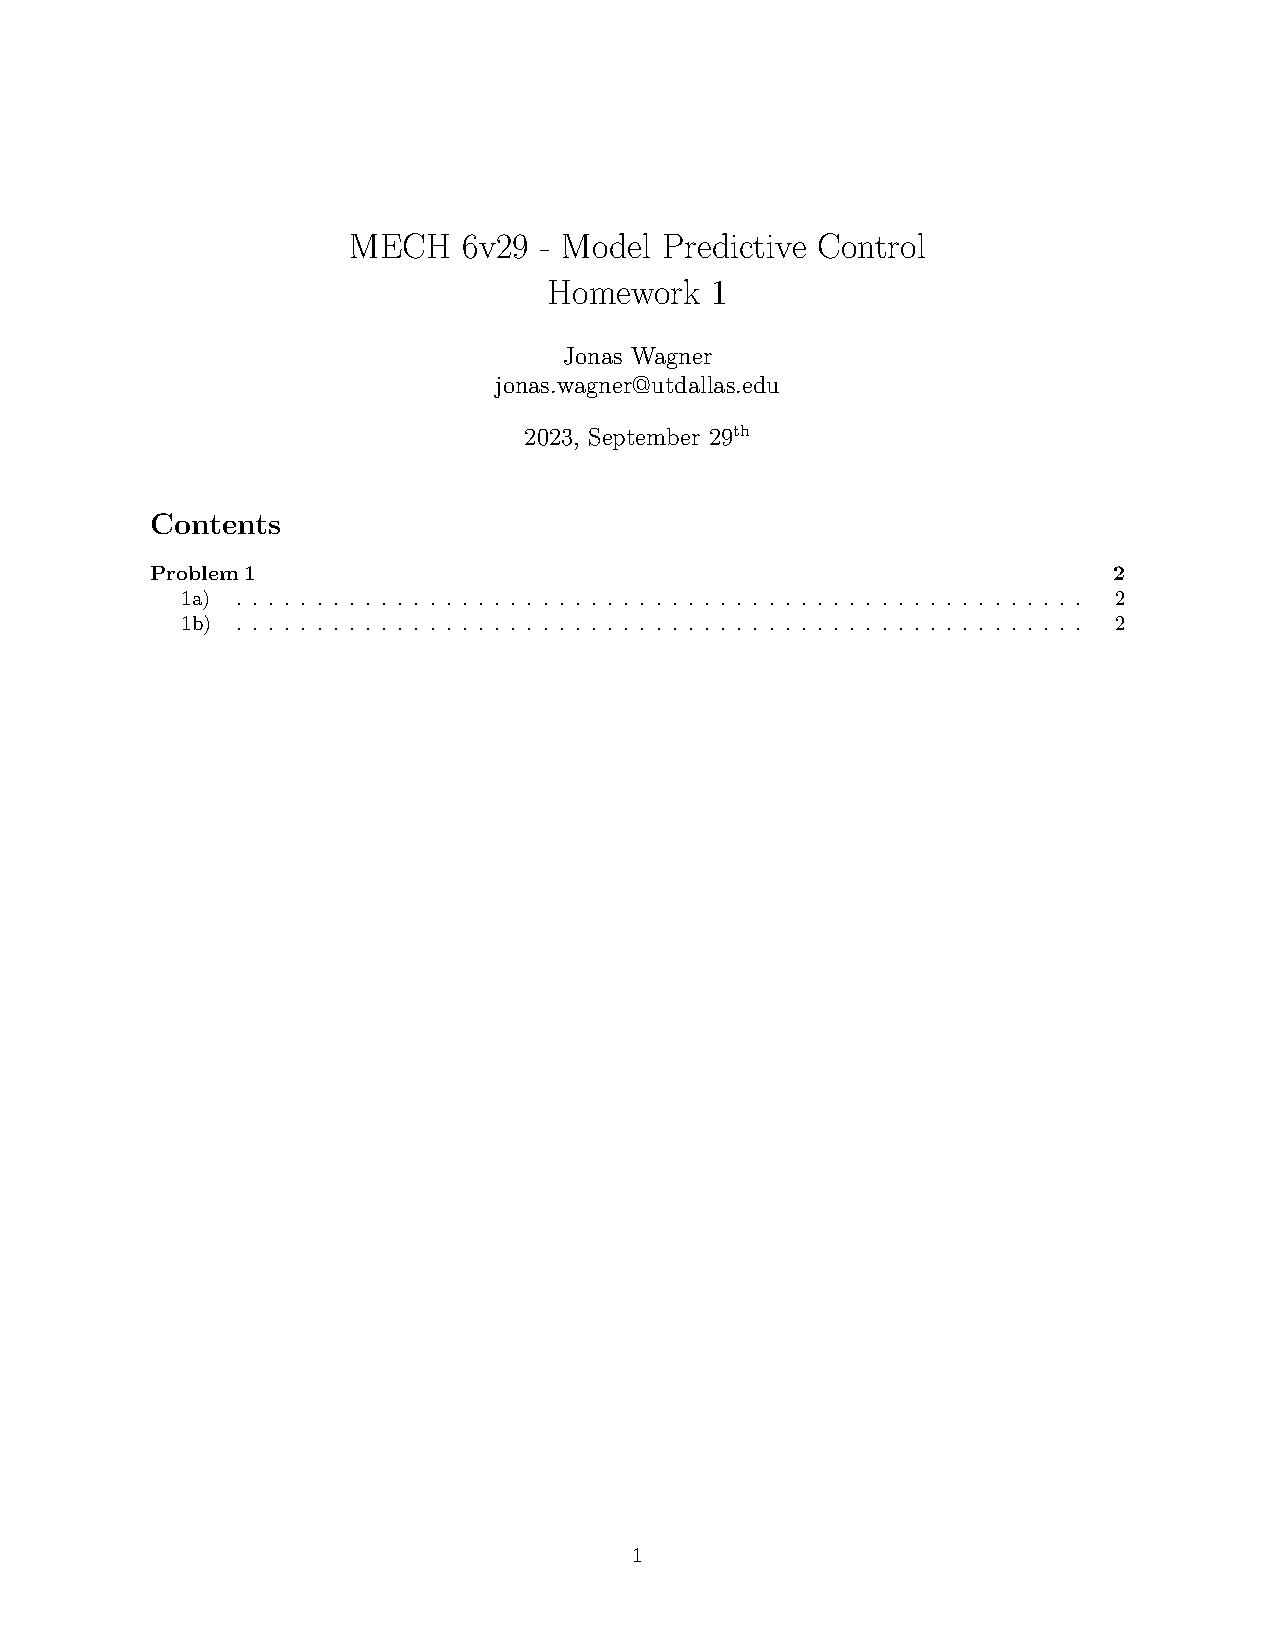
\includepdf[pages=-]{HW2.pdf}
% 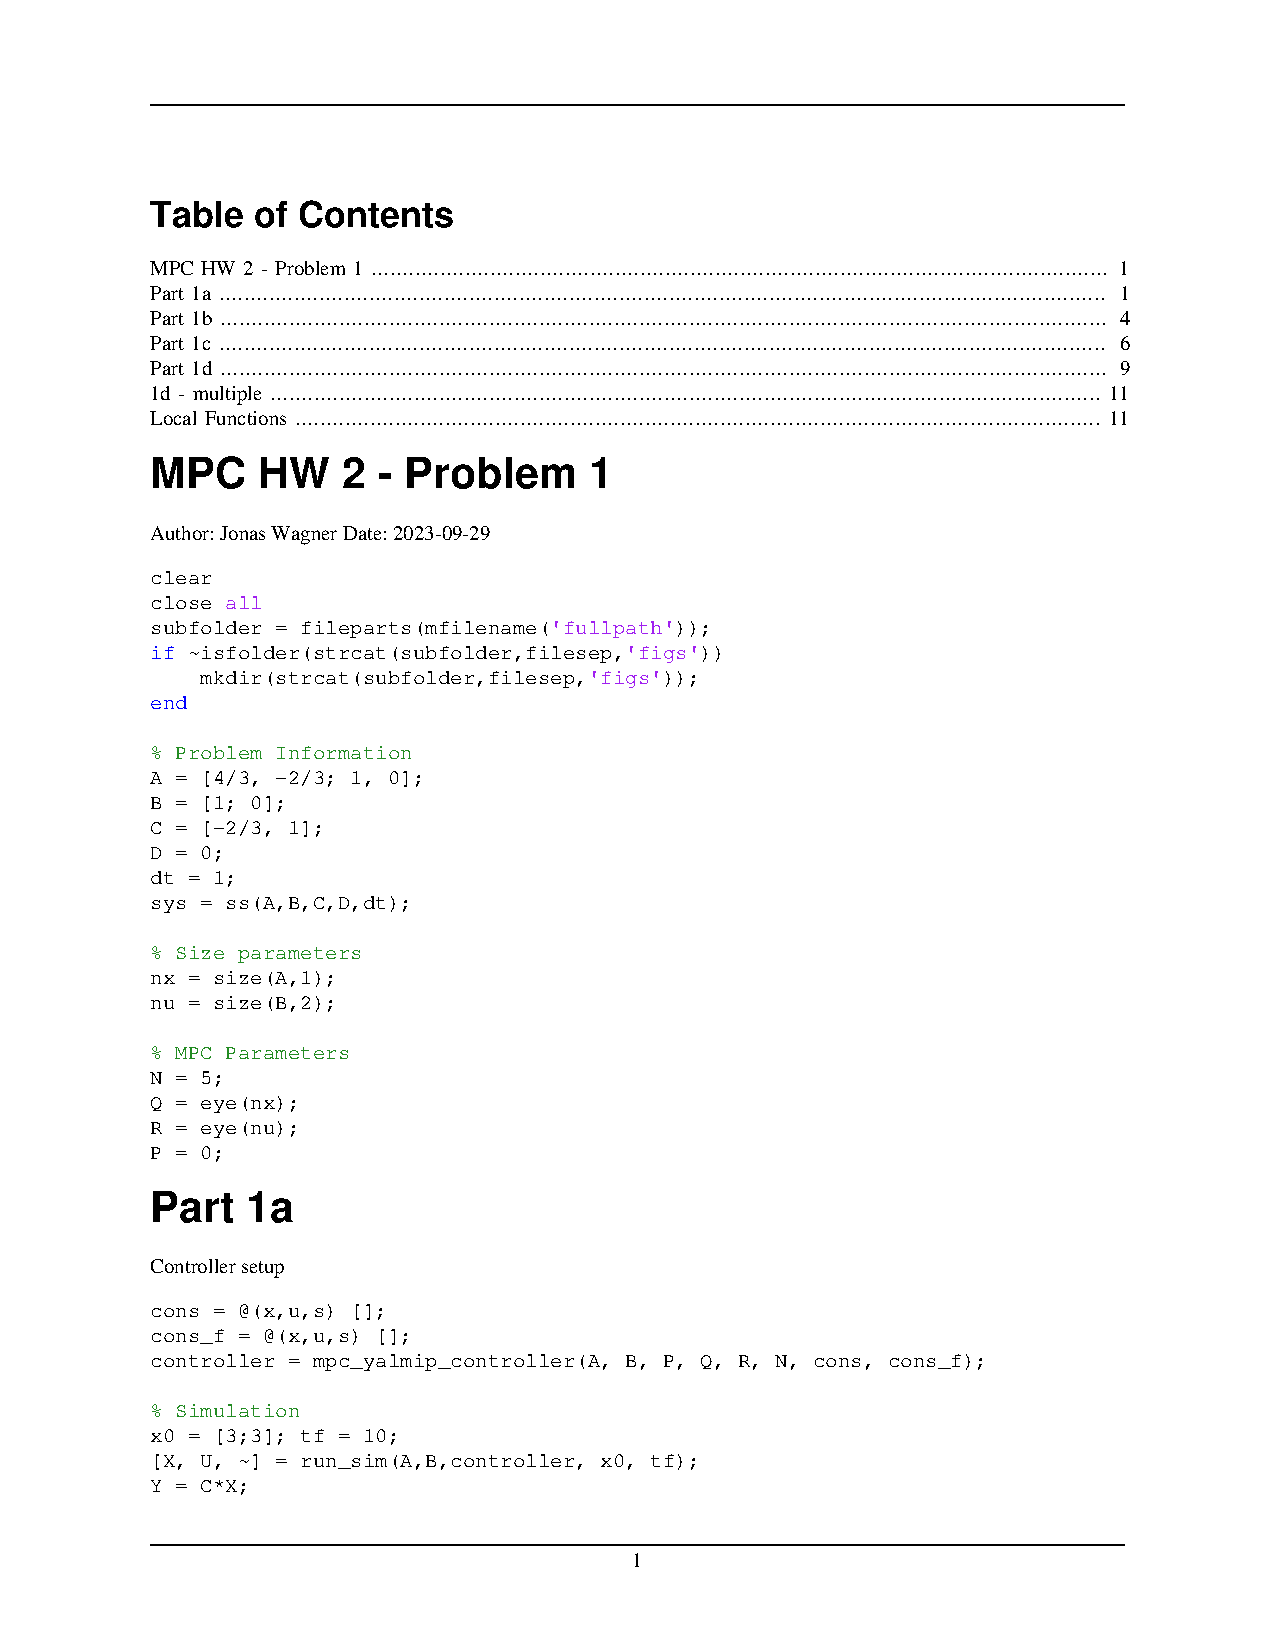
\includepdf[pages=-]{html/HW2_pblm1.pdf}
% 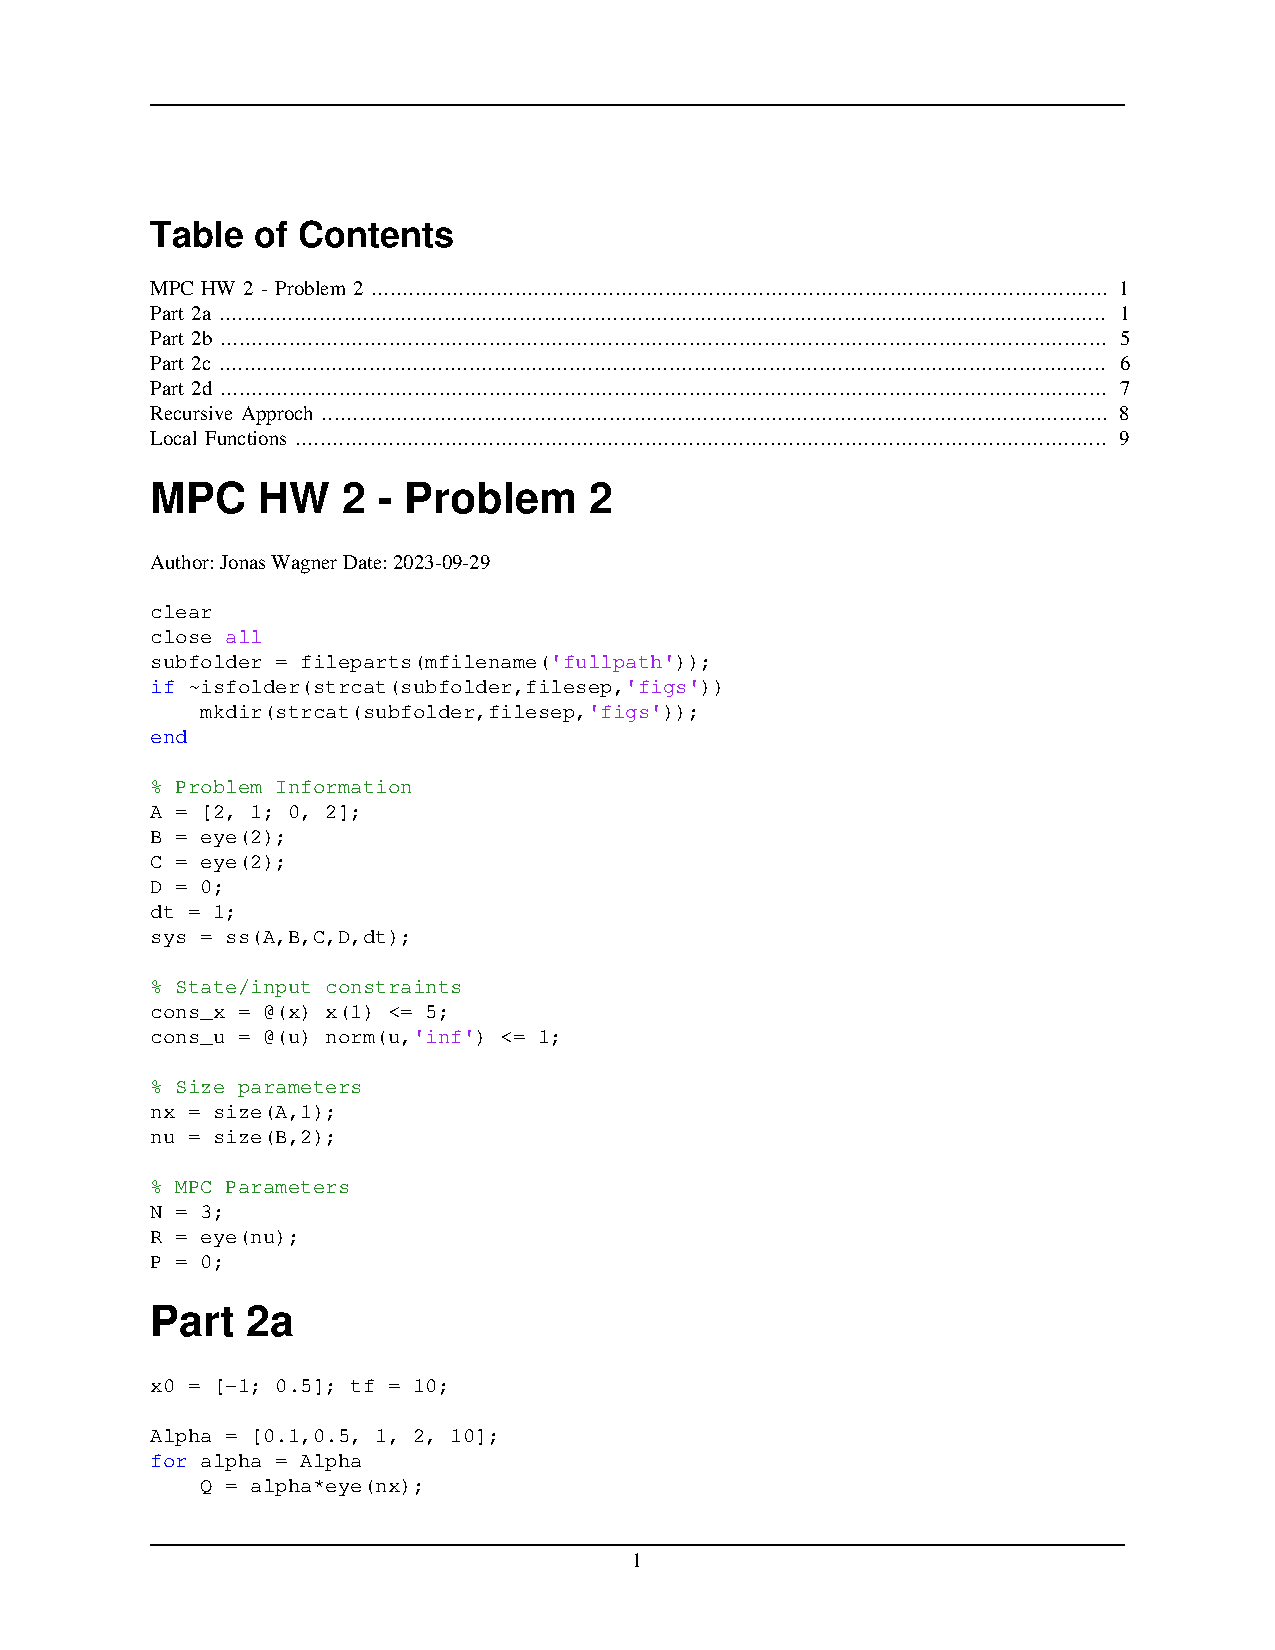
\includepdf[pages=-]{html/HW2_pblm2.pdf}


\end{document}
